% !TEX program = xelatex
\documentclass[
  10pt,
  twoside,
  openany,
  b5paper, % 以上均为 ctexbook 提供的文类选项
  colorscheme = basic, % 请根据需要选择或定制配色方案
]{qyxf-book}
\usepackage{pdfpages}
\usepackage[contents = 钱院学辅, scale = 15, color = black, angle = 50, opacity = .10]{background}
\includepdfset{pagecommand={\thispagestyle{plain}}}

\title{自然语言处理考纲·2020秋}
\subtitle{Syllabus of Natural Language Processing}  % 可选
\author{人工智能81王志博\ 钱龙}
\date{2021 年 2 月 3 日}
%\typo{AlphaGo}  % 排版人员信息,选填

% 定制元信息
\org{\Large\textit{钱学森书院学业辅导中心}\\\textsc{Qian Xuesen College Academic Counseling Center}}
\footorg{\textsc{Qian Yuan Xue Fu}}
\cover{
	\begin{tikzpicture}[remember picture, overlay]
		\begin{pgfonlayer}{background}
			\node at ($(current page.east)+(0in,0in)$){
				
\includegraphics[width=.8\textwidth]{cover.png} };
		\end{pgfonlayer}
	\end{tikzpicture}
}
\license{}  % 清空许可证信息

% 调整封面标题大小
\renewcommand{\titlefont}{\Huge\bfseries}
\renewcommand{\subtitlefont}{\LARGE\itshape}

\begin{document}
\maketitle
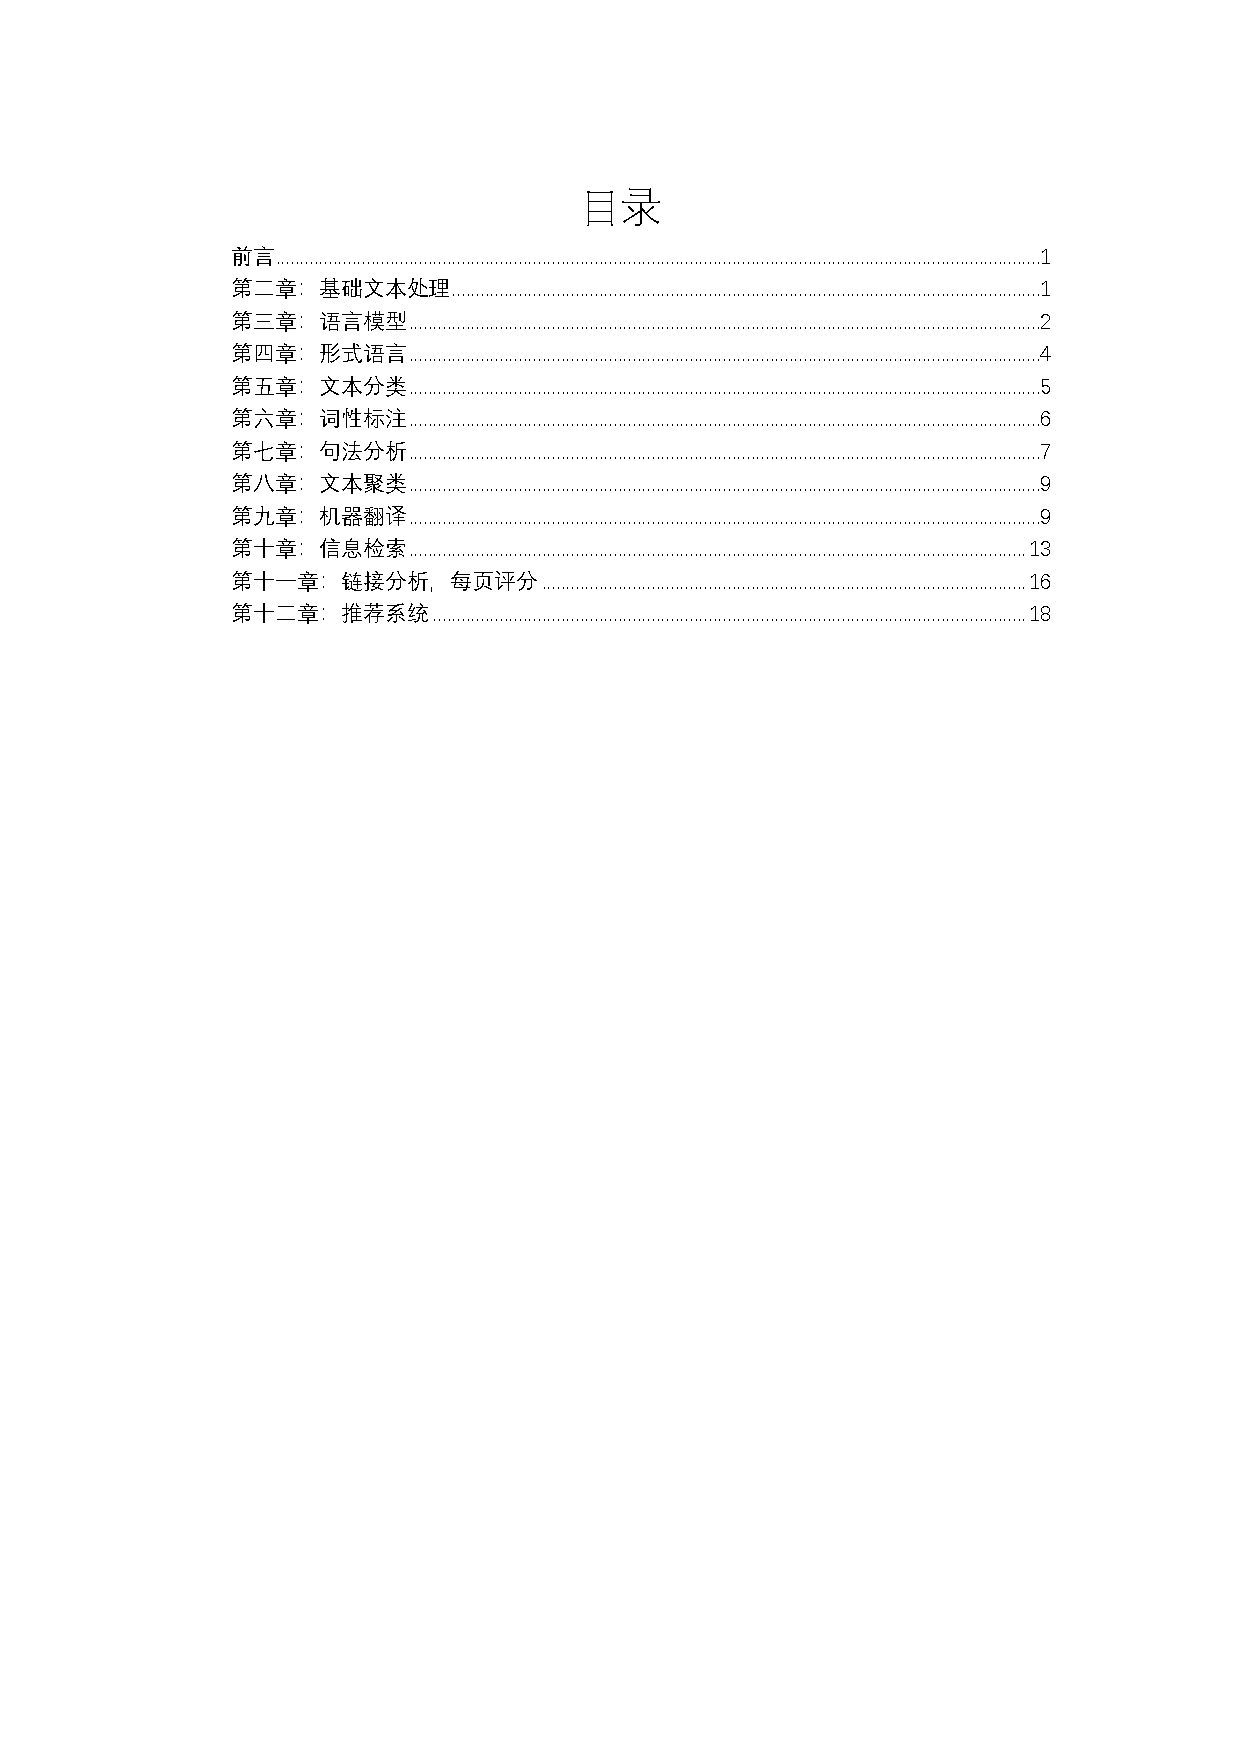
\includepdf[pagecommand = {\thispagestyle{empty}}, pages = - ]{toc.pdf}
\newpage
\setcounter{page}{1}
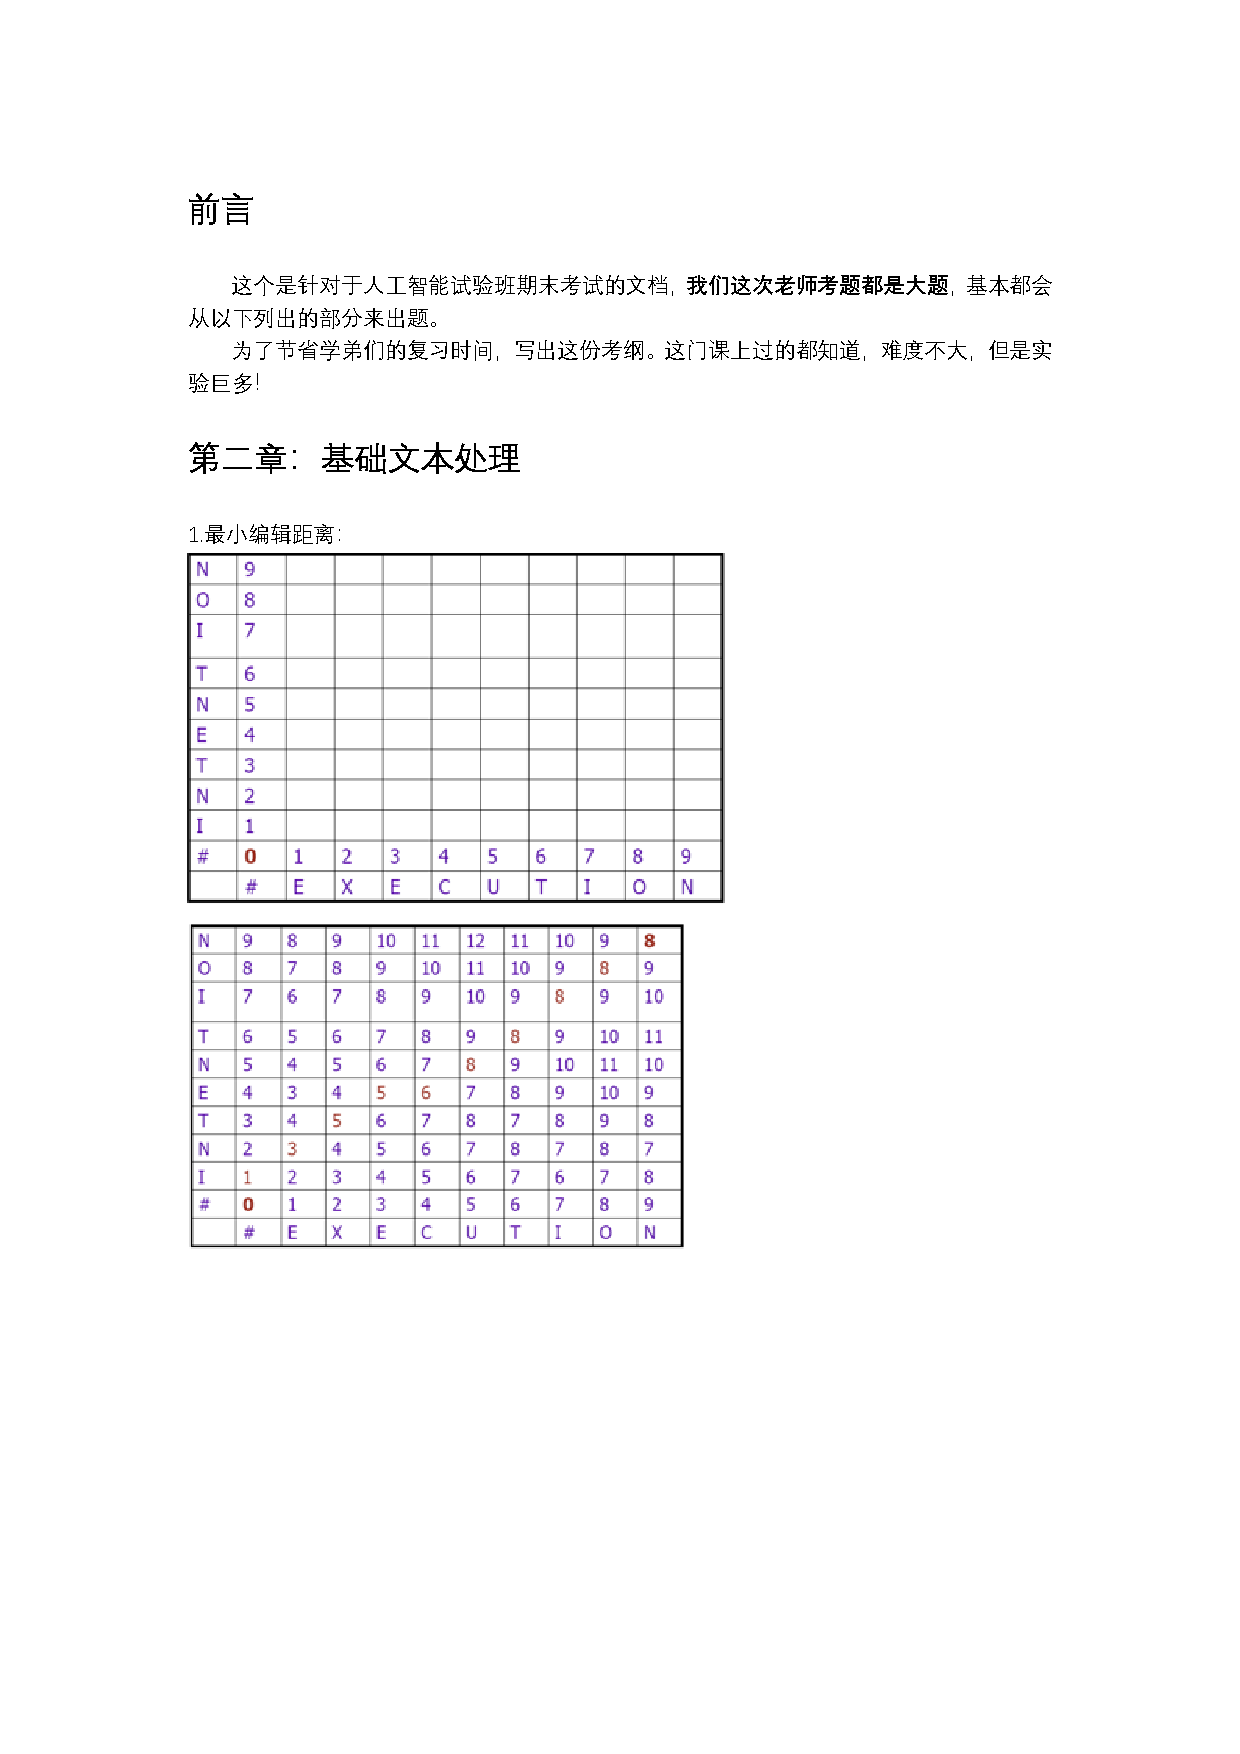
\includepdf[pages = - ]{content.pdf}
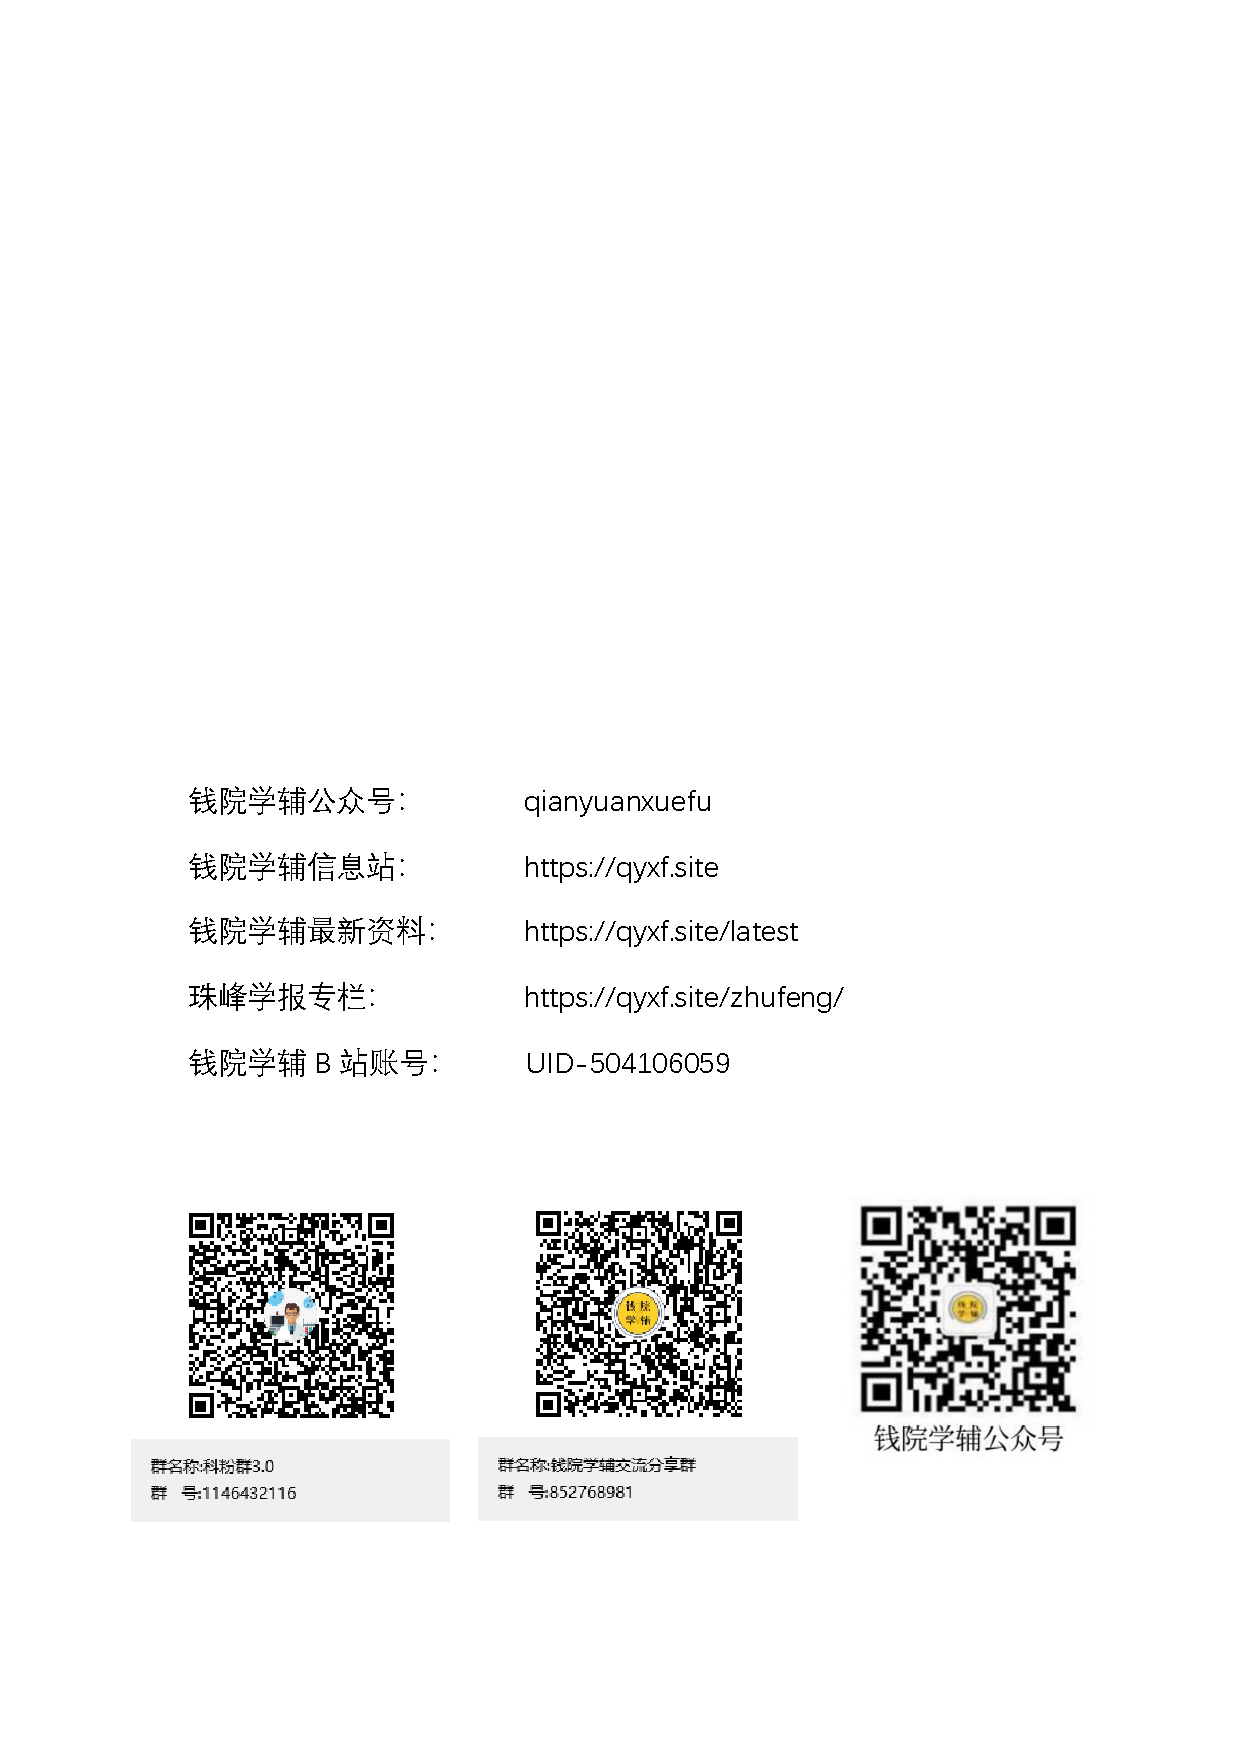
\includepdf[pagecommand = {\thispagestyle{empty}}, pages = - ]{lastpage.pdf}

\end{document}